\documentclass[12pt]{article}
\usepackage[a4paper, left=2cm, right=2cm, top=2cm, bottom=2.54cm]{geometry}


\usepackage[section]{placeins}
 
 
\usepackage[colorlinks, linkcolor=black, anchorcolor=black, citecolor=black]{hyperref}


\usepackage{titlesec}
\usepackage{titling}

\usepackage{xcolor}
 

\usepackage{biblatex}
\addbibresource{references.bib}

\usepackage{colortbl}
\usepackage[table]{xcolor}



\usepackage[export]{adjustbox} %for fitting the tables
 
 

 
\usepackage[nottoc,notindex,notlot,notlof]{tocbibind}
\usepackage{multicol}
\usepackage{minitoc}
\usepackage{multirow}
\usepackage{wrapfig}

\definecolor{Gray}{gray}{0.85}
\definecolor{LightCyan}{rgb}{0.88,1,1}


%\usepackage{times}


\usepackage[most]{tcolorbox}
\usepackage{hyperref} %For adding hyperlinks

%** new commands**%
\newcommand{\head}[1]{%
    \textcolor{white}{\textbf{#1}}}
\renewcommand{\arraystretch}{1.5}
\renewcommand*{\sectfont}{\bfseries}





\titleformat{\section}{\huge\scshape\raggedright}{}{0em}{}
  [\titlerule]
%\titleformat{\section}{\Large\bfseries\uppercase}{}{}{}[\titlerule]
\titleformat{\subsection}[runin]
  {\bfseries\large}
  {$\bullet$}
  {0em}{}[]
\titleformat{\subsubsection}[runin]
  {\bfseries}
  {}{0em}{}
  []
\titlespacing{\subsection}{.0em}{.45em}{1em}

\setlength{\parskip}{0.5em}
\title{Machine Vision in Agriculture}
\author{\textup{Pavan Kumar Kavvuri}}
\begin{document}
    \begin{titlepage}
\newcommand{\HRule}{\rule{\linewidth}{0.5mm}}

\includegraphics[width=8cm]{University_of_Bristol_logo.png}\\[1cm] 
\center 
\quad\\[1.5cm]
\textsl{\Large The University of Sydney}\\[0.5cm] 
\textsl{\large School of Chemical and Biomolecular Engineering}\\[0.5cm] 
\makeatletter
\HRule \\[0.4cm]
{ \huge \bfseries \@title}\\[0.4cm] 
\HRule \\[1.5cm]
\begin{minipage}{0.4\textwidth}
\begin{flushleft} \large
\emph{Author:}\\
\@author 
\end{flushleft}
\end{minipage}

\begin{minipage}{0.4\textwidth}
\begin{flushright} \large
\emph{Supervisor:} \\
\textup{Specify Your Supervisor}
\end{flushright}
\end{minipage}\\[3cm]
\makeatother
{\large An Assignment submitted for the UoB:}\\[0.5cm]
{\large \emph{Place Your Course Code and Course Name at Here}}\\[0.5cm]
{\large \today}\\[2cm] 
\vfill 
\end{titlepage}
    \newpage
    \section{Abstract}
    An accurate and reliable image based fruit detection system is critical for supporting higher level agriculture tasks such as yield mapping and robotic harvesting. Vision based 	fruit detection is a critical component for infield automation in agriculture. With accurate knowledge of individual fruit locations in the field, it is possible to perform yield 		estimation and mapping, which is important for growers as it facilitates efficient utilisation of resources and improves returns per unit area and time.
    
    Crop yield estimation is an important task in apple orchard management. Accurate yield prediction helps growers improve fruit quality and reduce operating cost by making 		better decisions on intensity of fruit thinning and size of the harvest labor force. It benefits the packing industry as well, because managers can use estimation results to 		optimise packing and storage capacity. Typical yield estimation is performed based on historical data, weather conditions, and workers manually counting apples in multiple 	sampling locations. This process is time-consuming and labor-intensive, and the limited sample size is usually not enough to reflect the yield distribution across the orchard, 	especially in those with high spatial variability. Therefore, the current yield estimation practice is inaccurate and inefficient, and improving it would be a significant result to the 	industry. 
    
    \newpage

\section{Introduction}

Robotics and Autonomous Systems (RAS) are set to transform global industries. These technologies will have the greatest impact on large sectors of the economy with relatively low productivity such as Agri-Food \cite{future_robotic_agri}.
The advent of autonomous system architectures gives us the opportunity to develop a new range of flexible agricultural equipment based on small, smart machines that reduces waste, improves economic viability, reduces environmental impact and increases food sustainability. Sensory data collected by robotic platforms in the field can further provide a wealth of information about soil, seeds, livestock, crops, flowers, fruits, costs, yield, farm equipment and the use of water and fertiliser to help farmers analyse data on weather, temperature, moisture, prices, etc., and provide insights into how to optimise yield, improve planning, make smarter decisions about the level of resources needed, and determine when and where to distribute those resources in order to minimise waste and increase yields\cite{views_forecasts}. This is termed as Precision Agriculture which concerns the use of monitoring and intervention techniques to improve efficiency, realised in application through the deployment of sensing technologies and automation.

Machine Vision offers significant opportunities enabling such intervention into precision agriculture, for example, crop monitoring, classifying when individual plants are ready for harvest\cite{article_Barnes}, work at night, quality analysis, detecting the onset of diseases etc. 
Despite these advances in agricultural automation that increased productivity by reducing manual labour and production costs, few agricultural tasks are still being handled manually, challenging the consistently shrinking and increasingly costlier agricultural labour force\cite{Kapach2012ComputerVF}. Probably, harvesting is the process that has received the least amount of technological development for satisfactory automation.\cite{article}.

Harvesting of delicate fruit, such as oranges,mangos, apples or peaches for the fresh market, is a process that cannot be performed using
aggressive methods such as shakers. This breaks down into 3 problems; firstly, building an autonomous navigating robot. Secondly, detecting and localising the ripen fruits on the tree and thirdly, selectively harvesting without harming other fruits. This report limits its scope to the study of automatic fruit detection and localisation problem.



Fruit picking(e.g berries), leaves harvesting(e.g tobacco), fruit counting and yield estimation etc, fall into this category. 
Machine vision in agricultural automation is yet to reach its full potential. Nonetheless, it has active applications in autonomous navigation and obstacles
avoidance (Astrand and Baerveldt, 2005; Wei et al., 2005; Zhao and Jiang, 2011),
precision and selective spraying (Berenstein et al., 2010; Tellaeche et al., 2008);
weed detection (Slaughter et al., 2008), yield estimation (Chinchuluun and Lee, 2006;
Qiao et al., 2005), seedling planting (Huang and Lee, 2010) and ripeness and quality
evaluation (Yongjie et al., 2010). Probably, harvesting is the process that
has received the least amount of technological development for satisfactory automation.\cite{article}

\\Harvesting of delicate fruit, such as oranges,mangos, apples or peaches for the fresh market, is a process that cannot be performed using
aggressive methods such as shakers. This breaks down into 3 problems; firstly, building an autonomous navigating robot. Secondly, detecting and localising the ripen fruits on the tree and thirdly, selectively harvesting without harming other fruits. This report limits its scope to the study of automatic fruit detection and localisation problem.

\\Currently the number of fruit on trees in a mango orchard is estimated via a manual count of a small number of trees to predict resource requirements for harvest, and to arrange marketing. Crop load is usually estimated at the stone hardening stage of fruit development, about six weeks prior to harvest, as at this stage the majority of fruit drop 	(fruit self-thinning) has occurred, and fruit numbers will remain relatively constant until harvest. How-ever, fruit colouration (anthocyanin synthesis, chlorophyll break-down) develops with further maturation on the tree.

However, this study dealt with fruit at close to harvest matu-rity, and consequently with more, and consistent, ‘blush’ (redcolouration) on the fruit than is found at the stone hardening stage.At stone hardening, fruit may be half green and half pale orange colour, or all green.\cite{PAYNE2014160}


\section{Aims and Objectives}
    
This project will focus on modern data processing techniques and segmentation techniques to facilitate precision agriculture in orchards. One desirable characteristic to measure is the number of fruits on a tree. By improving yield and fruit count estimates, growers can plan for harvest and also get information about the health of their crops. In the long run, this gives growers valued feedback about how efficiently they use resources, and how they can minimise the use of pesticides and fertilisers to
maximise their harvest \cite{stein2016improving}.

The aim of this project is to implement a machine vision algorithm for detecting and counting the number of fruits on tree crops. The objectives are to precise localise of fruits in the image and segment them out to perform the count. Questions to be addressed in while executing them are:
\begin{enumerate}
  \item How can we label the ripeness of the fruit in data?
  \item Will the algorithm disclose an occluded fruit?
  \item How can we precisely localise the fruit despite heavy leaf occlusions?
  \item How can fruit counts be isolated and associated to specific individual trees?
\end{enumerate}


\section{Motivation}

Crop yield estimation is an important task in apple orchard management. Accurate yield prediction helps growers improve fruit quality and reduce operating cost
by making better decisions on intensity of fruit thinning and size of the harvest labor force. It benefits the packing industry as well, because managers can use estimation results to optimize packing and storage capacity. Typical yield estimation
is performed based on historical data, weather conditions, and workers manually
counting apples in multiple sampling locations. This process is time-consuming
and labor-intensive, and the limited sample size is usually not enough to reflect the
yield distribution across the orchard, especially in those with high spatial variability. Therefore, the current yield estimation practice is inaccurate and inefficient,
and improving it would be a significant result to the industry. 





Traditionally, mapping of large farmlands and forests has been performed by using remote satellites and airborne sensing [17] [4]. Nowadays these methods have
a pixel resolution down to tens of centimeters1 which can be used to differentiate
individual trees. However, if to monitoring orchard health by parameters such
as stems, leaves and fruit, data is required to be measured at a much finer scale.
This is more readily achieved by ground vehicle based sensing or very close range
aerial platforms affording collection of higher resolution data.
Other advantages of ground based platforms include longevity of operation with
a wider range of sensors, this due to significantly higher power and mass budgets
than aerial platforms (though the aerial technology is rapidly improving), and
the potential for the technology to be deployed on existing farm infrastructure
such as tractors or other mobile machinery.
Current industry practice to estimate orchard fruit yield, involves assessment of
a manual field count. The number of trees to assess this count is often small e.g.
four across a total number of about a 1000 trees at the entire orchard. To attain
the total fruit count estimate, this average count is multiplied by the total number
of orchard trees [1]. However, the amount of fruit per tree is highly variable between trees, ranging from 20 to 200 mangoes. This makes the averaging method
inaccurate, and a poor estimate for the total orchard yield. Fruit counts should ideally also be assessed at several times during crop growth, which today is too
labour intensive, costly, and inefficient for farmers [1].

Nevertheless, farmers can use machinery to weigh and count the harvested fruit,
providing a size or weight distribution of individual fruit. However, both the
average method and this post-harvesting grading system give data about entire
orchard blocks. They can therefore not be used to map the distribution of yield
within a block which is critical for precision agriculture management.
The advantage of instead using a machine vision based system, is that it can facilitate fruit count estimates from a larger number of trees, could be used at individual trees, and at several times during the crop growth period.


\section{Related Work}
To satisfy our goals, the report deals
with the description of the main approaches developed by previous authors to automate the detection, localization and counting of fruits for automatic harvesting purposes.

Machine Vision based fruit yield estimation has been investigated for several years. To enable these estimates, both Unmanned Ground Vehicles and Unmanned Aerial Vehicles equipped with sensors like RGB, NIR and thermal cameras (uavs) have been used for image data collection of high value crops\cite{7294123}. The methods adopted by them investigate how to most robustly detect fruits in the images captured \cite{article_Stajnko} \cite{article_Linker}\cite{6697125}\cite{4781575}. 


the problem of creating a fast and reliable fruit detection system persists, as found in the survey by \cite{Kapach2012ComputerVF}. This is due to high variation in the appearance of the fruits in field settings, including colour, shape, size, texture and reflectance properties. Furthermore, in the majority of these settings, the fruits are partially abstracted and subject to continually-changing illumination and shadow conditions \cite{sa2016deepfruits}


Various works presented in the literature address the problem of fruit detection as an image segmentation problem (i.e., fruit vs. background). \cite{inproceedings_wang} examined the issue of apple detection for yield prediction. They developed a system that detected apples based on their colour and distinctive specular reflection pattern. Further information, such as the average size of apples, was used to either remove erroneous detections or to split regions that could contain multiple apples. Another heuristic employed was to accept as detections only those regions that were mostly round. \cite{bac2013robust} proposed a segmentation approach for sweet peppers.

Research on tree crop fruit yield estimates using machine vision have mainly been focusing on single view counts \cite{article_payne}, where the yield estimate is determined
as the total number of fruits visible in a single central, or two opposite views of the tree.

Current efforts on apple yield estimation using computer vision can be classified in two categories: (1) estimation by counting apples and (2) estimation by detecting flower density. A few researchers have worked on the first category using color images , hyperspectral images \cite{article_safren}, and thermal images.

Few studies aimed at modelling the correlation between flower density(as determined from image analysis) and fruit yield\cite{article_Aggelopoulou}.

The state-of-the-art object detection architecture, Faster R-CNN, is implemented in the context of fruit detection on
outdoor orchard images \cite{7989417_Bargoti}.  Detection is typically performed by transforming
image regions into discriminative features spaces and using
trained classifiers to associate them to either fruit or background objects such as foliage, branches and ground.

Semantic image segmentation performs this densely, resulting
in a pixel-wise classification over the image. Post-processing
techniques can then be applied to differentiate individual
whole-objects of interest as groups of adjacent pixels. On
the other hand, the detection search space can be reduced
using low-level image analysis to identify regions of interests
(RoIs) in the image (e.g. possible fruit regions), followed by
high-level feature extraction and classification.

Analysis of local colours and textures has been used for
pixel-wise mango classification, followed by blob extraction
to identify individual mangoes \cite{PAYNE2014160}.

More recently, Region based Convolutional Neural Networks (R-CNN) \cite{7112511_Girshick}, which combine the RoI approach
with CNNs, have produced state-of-the-art detection results
on PASCAL-VOC detection dataset \cite{everingham2010pascal}

\cite{sa2016deepfruits} recently demonstrated the use
of Faster R-CNN for sweet pepper and rockmelon detection
in a greenhouse and showed the versatility of the detector
amongst 5 other fruit types with images obtained from
Google Image search





\section{Risks Register}
   
\begin{table}[!h]
    \centering
    \sffamily
    \caption{Table variant 1} \label{tb:1}
    \begin{tabular}{|cccccc|}
        \rowcolor{black!75}
        \head{\#} & \head{Risk }& \head{Likelihood} & \head{Impact} & \head{Mitigation} & \head{Score}\\ 
        1 & Data quality & 0.5 & Affects the outcomes & ... & ...  \\ 
        \hline 
        2 & Top Layer & 1.4 mil &  \\ 
    \end{tabular} 
\end{table}



    
\section{Timeline}
    
\begin{figure}[!h]
  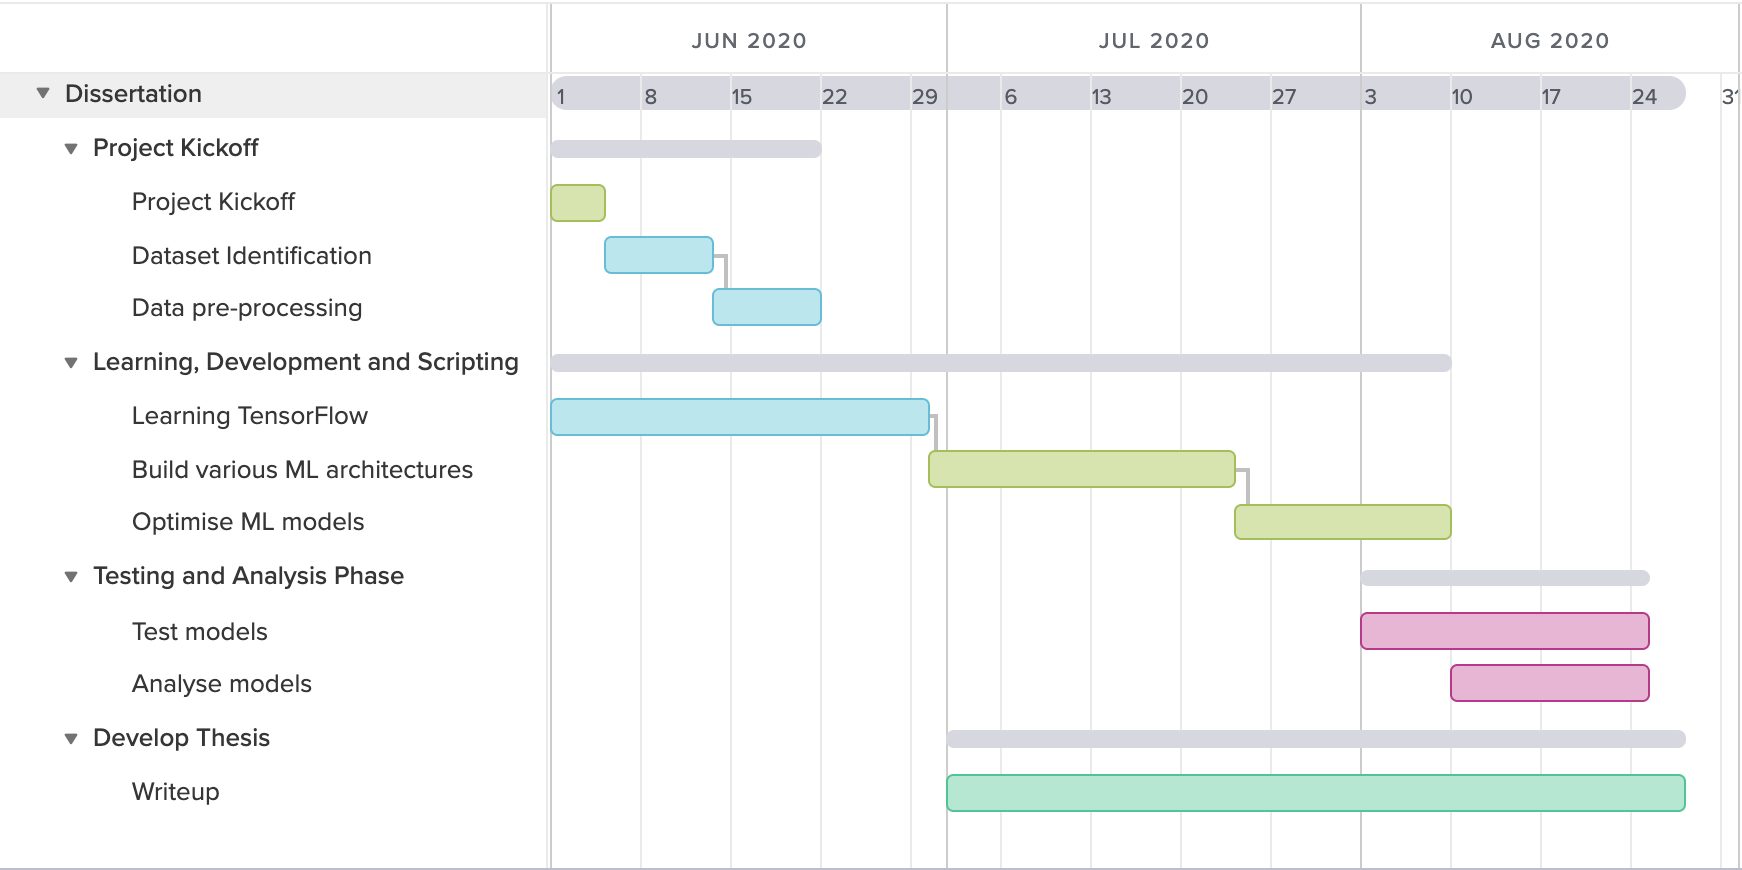
\includegraphics[width=\linewidth,scale=0.5]{timeline.png}
  \caption{dsadsadsa}
\end{figure}
    
  \newPage  
   
\printbibliography
 
  
    

\end{document}